\documentclass[11pt,a4paper]{article}
\newcommand{\ReportIdentity}{Experiment Report}
% Task-specific adaptation of the accepted Experiment Report typography.
% Shared P2 values remain editable only in the repository common source.
\usepackage[UTF8,fontset=none]{ctex}
\usepackage{fontspec}
\setmainfont{DejaVu Serif}\setsansfont{DejaVu Sans}
\setCJKmainfont{Noto Serif CJK SC}\setCJKsansfont{Noto Sans CJK SC}
\setCJKmonofont{Noto Sans Mono CJK SC}
\usepackage[a4paper,left=21mm,right=21mm,top=20mm,bottom=20mm,headheight=14pt,headsep=8mm]{geometry}
\usepackage{graphicx,booktabs,tabularx,array,amsmath,amssymb,longtable}
\usepackage{xcolor,titlesec,fancyhdr,caption,hyperref,microtype,placeins,float,etoolbox,enumitem,needspace}
% Smart Cities & Location Services — P2 Cloud Sorbet
% LOCKED visual palette v1 for Experiment Report
\definecolor{Paper}{HTML}{FCFAF7}
\definecolor{Ink}{HTML}{2D3238}
\definecolor{Muted}{HTML}{70757A}
\definecolor{P1}{HTML}{D3EAF5} % light blue
\definecolor{P2}{HTML}{F5D9B8} % apricot
\definecolor{P3}{HTML}{E8C7D3} % soft rose
\definecolor{P4}{HTML}{D7D3EA} % mist violet
\definecolor{C1}{HTML}{5B9FBE} % blue accent
\definecolor{C2}{HTML}{D49757} % apricot accent
\definecolor{C3}{HTML}{B97589} % rose accent
\definecolor{C4}{HTML}{8177A8} % violet accent
\definecolor{Rule}{HTML}{DDE3E7}
\definecolor{Panel}{HTML}{FFFDFC}

\pagecolor{Paper}\color{Ink}
\hypersetup{colorlinks=true,linkcolor=C1,urlcolor=C1,citecolor=C4,pdfauthor={吴博闻 / 10245102410}}
\linespread{1.18}\setlength{\parindent}{2em}\setlength{\parskip}{.25em}
\setlength{\emergencystretch}{2em}\clubpenalty=10000\widowpenalty=10000
\titleformat{\section}[hang]{\sffamily\bfseries\Large}{\color{C1}\fontsize{25}{27}\selectfont\thesection}{.65em}{}
\titleformat{\subsection}{\sffamily\bfseries\large}{\thesubsection}{.65em}{}
\titlespacing*{\section}{0pt}{1.3em}{.7em}\titlespacing*{\subsection}{0pt}{1.1em}{.5em}
\pagestyle{fancy}\fancyhf{}\fancyhead[L]{\sffamily\small\color{Muted}智慧城市与位置服务}
\fancyhead[R]{\sffamily\small\color{Muted}\ReportIdentity}\fancyfoot[C]{\sffamily\small\color{Muted}\thepage}
\renewcommand{\headrulewidth}{0pt}
\captionsetup{font=small,labelfont={bf,sf},labelsep=quad,skip=5pt}
\newcolumntype{Y}{>{\raggedright\arraybackslash}X}
\newcolumntype{L}[1]{>{\raggedright\arraybackslash}p{#1}}
\setlength{\tabcolsep}{4pt}\renewcommand{\arraystretch}{1.18}\setlist{nosep,leftmargin=2em}
\newcommand{\tabnote}[1]{\par\vspace{2mm}\begin{minipage}{\linewidth}\footnotesize\color{Muted}#1\end{minipage}}
\newcommand{\nextchapter}{\FloatBarrier\clearpage}\setcounter{tocdepth}{1}
\pretocmd{\subsection}{\Needspace{7\baselineskip}}{}{}\raggedbottom
\setlength{\textfloatsep}{13pt plus 2pt minus 2pt}\setlength{\intextsep}{11pt plus 2pt minus 2pt}
\newcommand{\reportcover}[3]{\hypersetup{pageanchor=false}\begin{titlepage}\thispagestyle{empty}\setlength{\parindent}{0pt}
\vspace*{21mm}{\sffamily\small\bfseries\color{C1}SMART CITIES \& LOCATION SERVICES}\par
\vspace{14mm}{\sffamily\fontsize{17}{23}\selectfont 任务分配实验}\par
\vspace{5mm}{\sffamily\bfseries\fontsize{27}{36}\selectfont #1}\par
\vspace{5mm}{\large #2}\par\vspace{17mm}{\color{Rule}\rule{\linewidth}{.8pt}}\par\vspace{12mm}
\begin{tabular}{@{}l@{\hspace{12mm}}l@{}}
\textsf{\textcolor{Muted}{姓名}}&吴博闻\\[2mm]
\textsf{\textcolor{Muted}{学号}}&10245102410\\[2mm]
\textsf{\textcolor{Muted}{课程}}&智慧城市与位置服务\\[2mm]
\textsf{\textcolor{Muted}{日期}}&2026年11月5日\\[2mm]
\textsf{\textcolor{Muted}{材料}}&实验二（1）与实验三学生版
\end{tabular}\vfill{\sffamily\small\color{Muted}#3}\par\vspace{4mm}
{\color{P1}\rule{.34\linewidth}{3pt}\color{P2}\rule{.22\linewidth}{3pt}\color{P3}\rule{.20\linewidth}{3pt}\color{P4}\rule{.14\linewidth}{3pt}}\par\vspace*{8mm}
\end{titlepage}\hypersetup{pageanchor=true}}
\newcommand{\datafigure}[3]{\begin{figure}[htbp]\centering\includegraphics[width=\linewidth]{../../figures/formal/#1.pdf}\caption{#2}\label{#3}\end{figure}}

\hypersetup{pdftitle={任务分配：在线匹配、多目标优化与强化学习}}
\begin{document}
\reportcover{在线匹配、多目标优化与强化学习}{从可信基线到结果驱动的优化与回退}{Experiment Report}
\pagenumbering{roman}
\section*{实验概述}
任务分配需要同时处理当前空间成本、没有到达的未来供需以及服务数量和收入之间的冲突。本报告分别构建单次在线二部匹配、静态多目标派单和跨时间片的车队仿真，先核验算法与指标，再进行成对控制变量和有限组合。结果显示，丢弃订单、混用离线目标和遗漏空驶成本都可能造成表面优势；增加算法复杂度也不一定带来额外收益。各项数值来自本轮实际运行，课件展示值仅作为教学参考。

基础部分沿用课件的物理尺度，同时单列Notebook的抽象尺度；进阶部分利用Foursquare签到构造出行代理\cite{teacher}。两类数据都不提供真实网约车业务效果的直接证明。最后的留出实验只确认预先冻结的方法，没有依据测试结果重新调参。
\tableofcontents\clearpage\pagenumbering{arabic}
\section{数据、尺度与研究问题}
\subsection{三种分配模型为何分开评价}
基础课件关注双边在线问题：司机和请求逐步到达，平台只看已发生事件，每个司机只用一次。静态多目标问题则把一个批次的全部司机和OD一次给出，允许主动不派，研究接驾与收入的前沿。强化学习问题允许同一辆车完成一次出行后继续接单，派单还会改变未来车辆位置。三者的信息、容量和时间语义不同，因此不能把静态NSGA的效用比直接当作在线延迟竞争比，也不能用一次批次的收入替代全天模拟收入。

\begin{table}[htbp]\centering\caption{保持独立身份的主要教学场景。}\label{tab:scales}
\begin{tabularx}{\linewidth}{lYYY}\toprule
场景&对象与时间&空间与速度&成本/目标\\\midrule
基础课件&20司机、20请求，0--20 min&10×10 km，1 km/min&等待+欧氏接驾时间\\
基础Notebook&100司机、100请求，0--2000时间单位&0--1000空间单位，速度1单位/单位&抽象单位的延迟\\
静态进阶&40司机、80代理订单&曼哈顿3 km候选半径，每单最多6司机&车费代理、接驾km、服务数\\
动态车队&40/60/100车，6:00--24:00&8×8网格，25 km/h，10 min/片&接单收入、应答、接驾和调度成本\\\bottomrule
\end{tabularx}
\end{table}

\subsection{Foursquare签到怎样成为代理订单}
两份教师压缩包及其嵌套归档含相同城市数据，逐字节哈希证实重复副本相同，不把它们累计成更多样本。Foursquare数据追溯至原作者发布页\cite{foursquare}。实收NYC有227,428条签到，TKY有573,703条；本次仿真按教师NYC矩形与模型展开，TKY用于完整来源、字段和质量审计，没有未经确认另建东京运营场景。数据包含用户、场所、类别、经纬度、UTC时间与逐条时区偏移。签到不是出租车订单，两个相邻签到也不提供实际道路或行程。

按教师代码，先取纬度$[40.60,40.88]$、经度$[-74.05,-73.75]$内签到，再按用户和当地civil-clock排序。同一当地日期内，相邻保留签到间隔10--180 min、曼哈顿工作距离至少1 km时形成一个OD代理，得到25,550条。先做矩形筛选再相邻配对可能跨过矩形外的记录，这是代理机制的局限。

工作坐标为$x=(\mathrm{lon}+74.05)\,111\cos40.74^\circ$、$y=(\mathrm{lat}-40.60)\,111$，以教学近似km计算。文件没有独立的datum证明，因此不将该模型解释为已确认的绝对地理精度。进阶车费代理为$5+2d_{OD}$，基础NSGA只用欧氏送客距离表示收入，二者不混用。

\subsection{时间审计与训练、选择、确认}
每条UTC加该记录的分钟偏移形成当地时间。独立取回OD两端的原始来源行后发现，12对的UTC实际间隔与当地钟面差不一致，其中6对UTC倒序，且12对都不满足UTC的10--180 min窗口。因此主基线准确称为教师local-clock代理，不能据此断言真实出行时长。保留原始值，另以剔除这12对的副本做训练内稳健性，不静默更换数据定义。

按代理记录的不同日期排序，前70\%日期为训练大区间、后30\%保持测试；训练大区间的后20\%日期用作验证，前段为inner训练。对应inner有19,617条/139个日期，验证1,972条/35个日期，测试3,961条/75个日期；分界分别为2012年10月19日与11月27日。模拟日从相应池中重采样1500单，训练300回合是300次仿真，不能写成300个真实运营日。

原Notebook从全量签到采样司机热点，会让未来测试位置进入训练条件。本次将开发的初始司机严格限制到inner签到，最终重训后只用前70\%签到。验证用于选择，测试只作冻结后的确认；用于全量描述的统计不当作训练特征。两城市原始数据中的重复、起止日期与作者网页/README差异均保留审计，不根据课件参考条数修改源文件。

\begin{figure}[htbp]\centering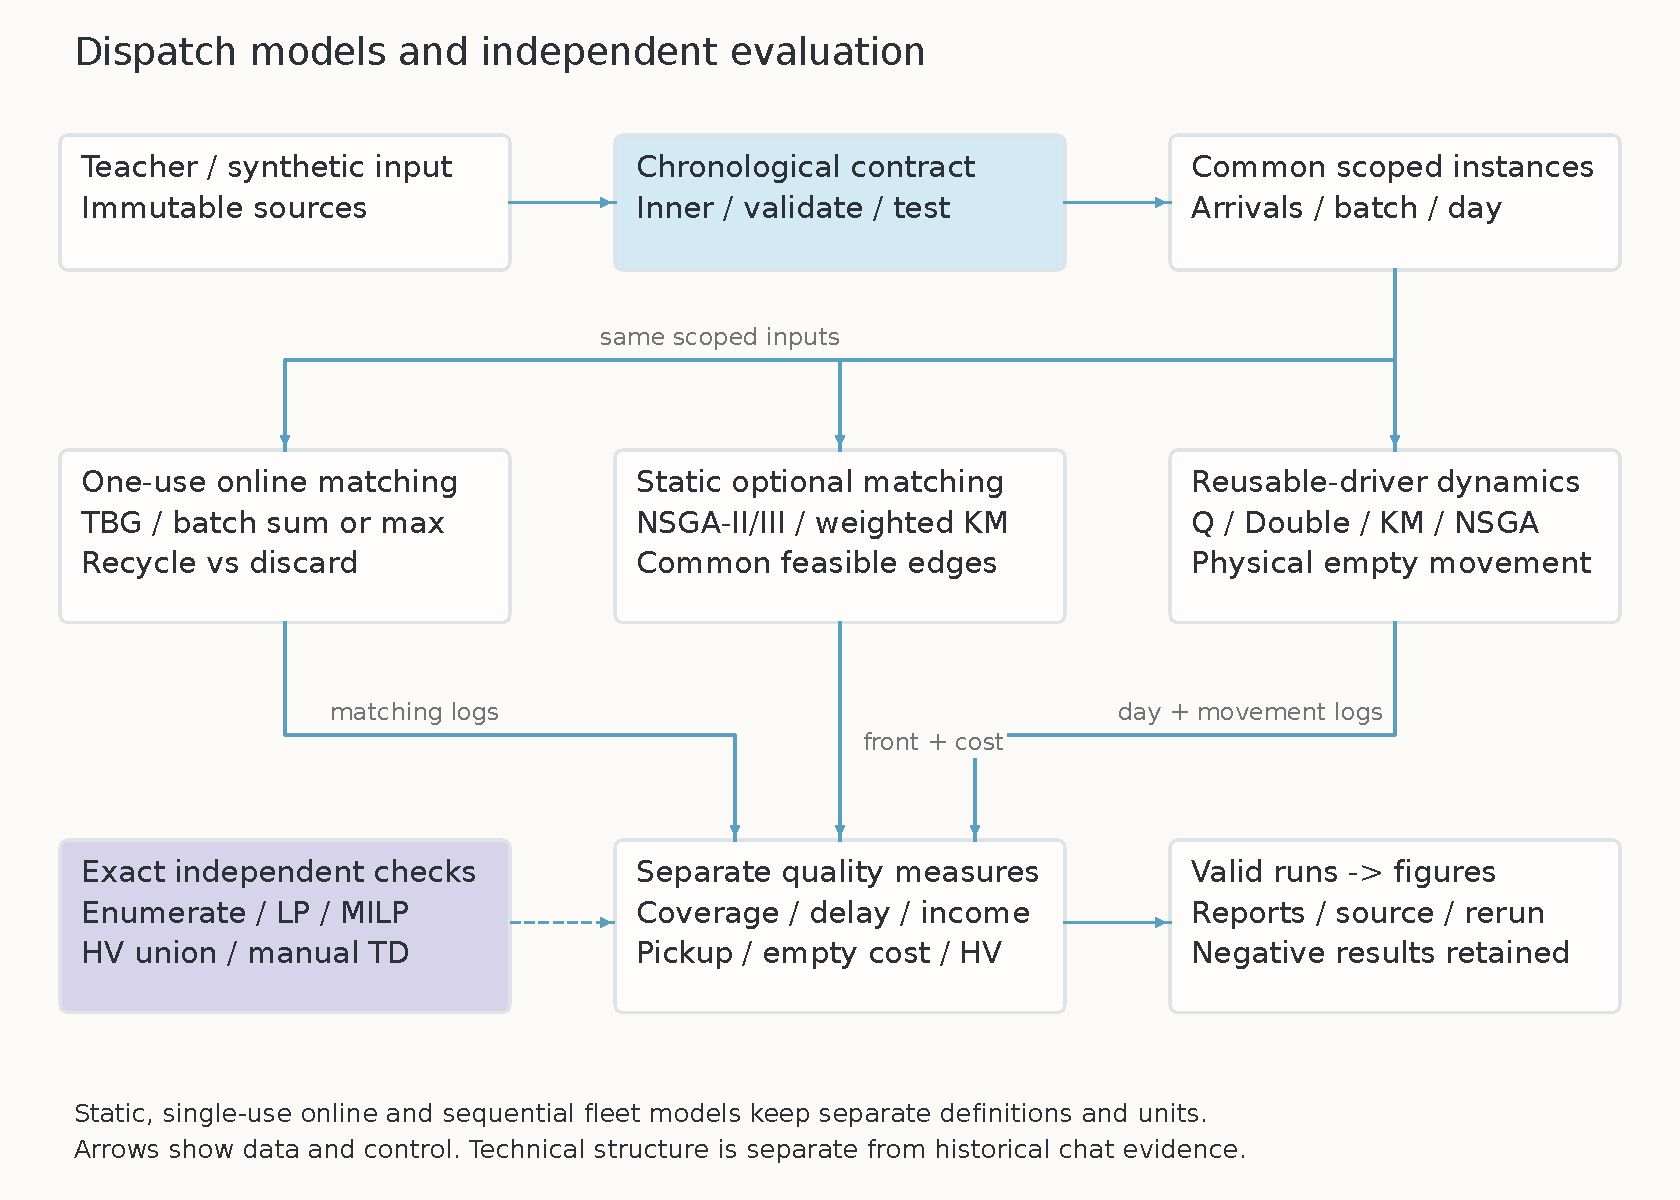
\includegraphics[width=\linewidth]{../../diagrams/dispatch_runtime_and_evaluation.pdf}
\caption{本次实现的三个模型与共同核验关系。静态、单次在线和跨时间车队采用不同容量语义，参考求解器与结果指标分开。图中箭头表示实际技术依赖。}\label{fig:runtime}\end{figure}

\nextchapter\section{在线派单：覆盖率、平均与最差体验}
\subsection{事件、阈值与结束行为}
Worker和Request均有唯一ID、坐标和到达时刻；同刻先处理请求、再处理司机，各自按ID稳定排序。BB在同刻全部到达后才执行该时刻的批次；结束时补最后非重复批次。派单不早于双方可用，接驾可以在仿真horizon之后完成。对请求$r$和司机$w$，
\begin{equation}
D_{wr}=(t_{assign}-t_r)+\frac{\lVert x_w-x_r\rVert_2}{v}.
\end{equation}
第一项是乘客已等时间，第二项是接驾行驶时间；分别保存，不用单一总数隐藏机制。

若只考虑当前接驾距离，可设计“在已到达且可行的司机中取最近者”的在线贪心；对一个已知批次则用最小总距离匹配优化整体和，若关心最差体验就改求瓶颈。最近的局部选择不保证未来全局最优，这也是继续比较TBG和批次策略的原因。

TBG的$\gamma$是时间阈值。请求到达时，在已到司机中取行驶时间不超过$\gamma$的最近者，否则缓冲。司机到达时先服务FIFO首个等待$\ge\gamma$的请求，不再限制距离；没有超时请求才在总延迟$<\gamma$的候选中取最小者，否则司机缓冲。该行为按本轮提示词和Notebook实现；课件伪码的严格/非严格边界与Notebook有差异，不能悄悄混合。结束兜底只匹配真实剩余双方，供给不足明确保留未服务对象。

BB每隔$\theta$对缓冲双方匹配。Notebook的线性分配最小化总延迟，课件另提最小最大延迟，故分别标为BBsum和BBmax。正式版本回收未匹配对象；原starter清空双方的discard策略作为单独对照。半径或容量等约束可通过共同可行边与顶点容量表达；没有可行边就不匹配，不能强行连边凑满服务数。

\subsection{用什么离线参考计算实例比值}
完全知道未来时，单次匹配每条边的最早派单为$\max(t_w,t_r)$，成本$C_{wr}=\max(t_w-t_r,0)+d_{wr}/v$。先固定最大可行基数$k$，再分别求$\min\sum C$和$\min\max C$。前者使用线性分配\cite{scipy}，后者对边成本阈值做最大基数可行性检查。

例如$C=\left[\begin{smallmatrix}0&6\\6&10\end{smallmatrix}\right]$，sum最优取对角线，总10、最大10；瓶颈最优取非对角线，总12、最大6。调用KM不能自动证明最差延迟最优。小图枚举、独立线性规划与另写二部可行性程序核对了两种参考。

在线目标值除以同实例、同基数、同目标的离线值，才得到本报告的实例比值。零分母、无匹配和基数不同均保留不可计算状态，不能填0或把不完整服务与全服务最优直接相除。有限输入上的实测比值也不构成全输入空间的理论竞争保证。

\subsection{丢单为何会制造较好的条件延迟}
\begin{table}[htbp]\centering\small
\caption{五个开发实例：覆盖和延迟必须一起解释。}\label{tab:onlinedevelopment}
\begin{tabularx}{\linewidth}{Yrrrrr}\toprule
方法(参数) & 匹配率 & 均值/min & 最大/min & P95/min & max实例比\\\midrule
TBG(2) & 1.00 & 7.399 & 13.342 & 11.876 & 1.649\\
TBG(5) & 1.00 & 5.119 & 12.802 & 12.119 & 1.568\\
BBsum(1) & 1.00 & 5.748 & 15.426 & 12.157 & 1.872\\
BBmax(1) & 1.00 & 5.965 & 14.598 & 12.023 & 1.794\\
discard(0.5) & 0.25 & 4.379 & 6.516 & 6.316 & --\\
离线sum & 1.00 & 4.103 & 11.487 & 9.412 & 1.406\\
离线max & 1.00 & 5.747 & 8.370 & 8.145 & 1.000\\
\bottomrule\end{tabularx}
\tabnote{每行对5个输入seed先逐实例算指标，再平均；P95不是把全部seed混成单条观测。部分覆盖的实例比无定义，以--表示。}
\end{table}

教师20×20场景的五个开发seed中，$\theta=0.5$的discard平均覆盖25\%，回收版本覆盖全部请求；司机先到而请求后到的场景中，discard甚至完全没有服务。因此图\ref{fig:onlinecdf}以全部请求为分母，未匹配质量留在较低平台。另一半图用每个实例的平均与最大延迟成对展示：改善均值不自动改善尾部。

\datafigure{online_delay_and_coverage}{教师物理场景，5个成对输入seed、每seed20请求。左侧每点是一个实例，十字为跨seed均值；右侧分母100请求，黑线为discard，覆盖25\%。}{fig:onlinecdf}

\subsection{阈值、到达顺序与局部瓶颈的边界}
原始控制变量包含供需比、热点、司机/请求先到、规模与批长；同一因素变化以相同输入和成对seed比较。教师场景中TBG小阈值0.5/1/2均有平均17\%服务推迟到结束兜底，阈值5下降到7\%，但阈值继续增大并不保证更低最大延迟。由这一观察触发3种到达顺序下的局部阈值实验（图\ref{fig:gamma}），而非预先堆叠增强。

\datafigure{online_threshold_diagnosis}{阈值的针对性开发实验。每点为5个相同输入seed的均值，误差条为seed标准差；右侧是结束兜底比例。线只连接实测阈值。}{fig:gamma}
\datafigure{online_spatial_mechanism}{同一教师实例的空间匹配与等待/行驶分解。案例按TBG5最大延迟中位seed选择；连线是接驾边，不代表真实道路。每个面板均使用同一20对输入。}{fig:spatial}

BBmax在一个批次内最小化最大成本，但会改变留给未来的司机。开发teacher seed13中，$\theta=1$的BBmax全天最大延迟反而比BBsum高2.162 min，不能把局部数学最优扩大为整个在线过程保证。供需不平衡和到达顺序也改变阈值的作用（图\ref{fig:scenes}）。没有对这些负例改写指标。

\datafigure{online_scenario_matrix}{6种真实运行场景、5seed均值，颜色表示同基数的最大延迟实例比值，越小越好。每格是实测设置，没有插值。}{fig:scenes}
\begin{table}[htbp]\centering\small
\caption{五个独立合成确认实例：不按结果重新选择阈值。}\label{tab:onlineconfirmation}
\begin{tabularx}{\linewidth}{Yrrrrr}\toprule
方法(参数) & 匹配率 & 均值/min & 最大/min & P95/min & max实例比\\\midrule
TBG(2) & 1.00 & 7.639 & 13.581 & 13.007 & 1.936\\
TBG(5) & 1.00 & 5.411 & 15.927 & 14.070 & 2.272\\
BBsum(1) & 1.00 & 5.255 & 12.208 & 10.111 & 1.727\\
BBmax(1) & 1.00 & 5.369 & 12.208 & 10.291 & 1.727\\
discard(0.5) & 0.37 & 5.348 & 9.239 & 8.808 & --\\
离线sum & 1.00 & 4.033 & 10.645 & 7.863 & 1.497\\
离线max & 1.00 & 5.136 & 7.050 & 6.914 & 1.000\\
\bottomrule\end{tabularx}
\tabnote{每行对5个输入seed先逐实例算指标，再平均；P95不是把全部seed混成单条观测。部分覆盖的实例比无定义，以--表示。}
\end{table}

独立合成确认使用seed110--114，没有据其结果再选阈值。TBG5的平均延迟5.411 min低于TBG2的7.639 min，但平均最大延迟15.927 min高于13.581 min：开发样本中阈值5对尾部的轻微优势没有在确认样本保持。因此不把阈值5推荐为普适改进；平均与最差体验仍需分别判断。结论只适用于所列到达和空间模型。

\subsection{真实签到对空间需求的扩展}
从inner训练的4个小时池重采样20个代理起点，形成各自60 min流；司机位置也只取训练签到，司机到达时间为模拟值。空间采用原条件工作坐标、速度1 km/min，与10×10 km均匀教学场景分开标识。图\ref{fig:proxyhours}比较时段和方法，不把重采样批次称为真实运营小时。
\datafigure{online_proxy_hours}{8/13/18/23点来源的历史代理起点，各5个采样seed。左、右分别为已匹配平均延迟和最大延迟，20司机/20请求；教学局部km与模拟分钟。}{fig:proxyhours}

\nextchapter\section{多目标优化：前沿形状与初始化}
\subsection{先定义可行解和收入，才比较算法}
基础NSGA单独运行20司机/20合成OD，10×10 km欧氏空间；两个目标为最小总接驾距离与最大总送客km，不引入进阶车费。所有边可行，匹配可选；每个固定$\lambda$按$U=\sum d_{OD}-\lambda\sum d_{pickup}$选解，与完全相同可行图的精确最大效用KM比较。五seed结果及前沿见图\ref{fig:basicfront}。该静态效用实例近似比为$U_{OPT}/U_{EA}$，不同于上一节在线延迟比；无标量偏好的一整条Pareto前沿没有唯一竞争比。
\datafigure{evolution_basic_scalar_reference}{基础部分独立的欧氏OD实验，五个进化seed，100种群/300代。车费目标仅为送客km；标量化参考来自同一可行图的精确求解，不是在线理论界。}{fig:basicfront}

进阶整数编码长度为订单数，第$j$位0表示不派，其余值指向该单最近K个可行司机；按请求顺序解码，司机冲突时轮转候选，耗尽则不派。所有算法共享这个半径/候选图与单次容量。统一最小化目标$F=(-\sum fare,\sum pickup)$，第三目标加入$-\#served$，因此空匹配是合法端点，不用伪造服务数提高收入。

\subsection{非支配保留和共同评价标尺}
NSGA-II以非支配层、逐目标归一化拥挤距离和精英保留筛选\cite{nsga2}；NSGA-III保留非支配层，把临界层截断换成理想点/超平面归一化、参考方向关联和小生境保留\cite{nsga3}。这些机制按教师整数编码作教学实现。二目标100种群/100方向；三目标按Notebook的105种群/105方向，奇数种群必须生成实际105个子代而非104个。交叉概率0.9，每位变异概率$1/m$；100种群/300代的实现实际评价30,100个个体（包括初代）。

HV使用所有方法共同的预先界：收入上界由同可行图精确最大收入匹配求得，接驾上界为容量×3 km，第三目标服务上界为容量；各维归一化后参考点统一1.1。HV可大于1，因为参考盒边长1.1，而不是把它解释为百分比。Spacing采用不同规范非支配点之间最近L1距离的变异系数；不足两点或均距0时无定义。

独立审核发现，加权KM的离散权重输出可能包含支配点，以及求和次序带来的约$10^{-13}$差异。保留原始输出，报告端对所有方法统一按10位小数规范去重后取非支配集；8/10/12位敏感性与另写box-union核验确认其影响范围。不能只对某一个算法换标尺使其看起来更好。

\datafigure{evolution_front_and_convergence}{18点inner训练批次，5个进化seed；共同可行边与固定HV标尺。收敛阴影为5seed最小--最大范围，KM只求离散权重方向，不保证完整前沿。}{fig:frontconv}
\begin{table}[htbp]\centering\small
\caption{18点相同开发批次；5seed均值±样本标准差，DTLZ2独立使用92/400设置。}\label{tab:evobaseline}
\begin{tabularx}{\linewidth}{Ylrrr}\toprule
问题 & 算法 & HV & Spacing & EA秒\\\midrule
派单2D & NSGA-II & 1.090244 $\pm$ 0.004460 & 0.505 & 2.455\\
派单2D & NSGA-III & 1.077092 $\pm$ 0.009530 & 0.938 & 3.601\\
派单3D & NSGA-II & 1.014845 $\pm$ 0.010260 & 0.621 & 2.560\\
派单3D & NSGA-III & 1.012638 $\pm$ 0.005689 & 0.688 & 4.220\\
DTLZ2 & NSGA-II & 0.707111 $\pm$ 0.006190 & 0.480 & 1.087\\
DTLZ2 & NSGA-III & 0.744325 $\pm$ 0.000235 & 0.297 & 1.841\\
\bottomrule\end{tabularx}
\tabnote{各问题使用各自预先定义的共同标尺，HV不是百分比，也不跨不同问题比高低。}
\end{table}


\subsection{加权和何时遗漏，三目标何时需要参考方向}
在该离散派单问题中，加权和KM能高效找到很多supported解，尤其补足高收入端；但非凸部分的unsupported解不可能成为某个线性权重最优。一个已知答案的最小化例子是$(0,2),(1,1.1),(2,0)$：中点不被支配，却无法胜过两端的加权和最优。这里还有限权重网格的覆盖问题，即便supported解也可能漏掉，不能把两种原因混为一谈。

三目标派单中的服务数与收入高度相关，前沿可能仍很窄；目标维数增加不保证NSGA-III胜出。DTLZ2提供真正铺开的球面几何，图\ref{fig:three}与图\ref{fig:dtlz}并置说明参考方向的适用差异。DTLZ2使用教师给定的离散编码实现及独立公式参考，不把它冒称任意连续全局优化保证。Spacing是局部分布离散度，需与HV、端点、误差一起判断。

\datafigure{evolution_three_objective_geometry}{实际三目标派单前沿：负号转换回正收入/服务数展示，三维和二维投影互为补充。第三维是真实服务数。}{fig:three}
DTLZ2五seed的平均球面径向误差$|\lVert F\rVert_2-1|$分别为II $0.0076465\pm0.0013867$、III $0.00007084\pm0.00005153$（样本标准差）。这项有已知球面参考的误差与Spacing提供互补信息。
\datafigure{evolution_dtlz2_geometry}{DTLZ2的seed0实测点与解析球面网格；多次运行的径向误差见正文，分布统计见表。5seed统计与派单场景独立，不能直接比较不同实例的绝对HV大小。}{fig:dtlz}

\subsection{先增加预算，再测试KM种子}
基础18点结果的高收入端不足，先比较种群200/代数300，以及种群100/代数600，二者约60,000次评价。随后保持原100/300预算，插入最多10个真实编码的KM解，其余仍为原初始化；验证$decode(encode(KM))$与原匹配完全一致。初始化额外41次标量求解、41次目标求和和耗时单列，没有藏在EA计时之外。

观察到KM初始化稳定改善端点和前沿后，才组合KM初始化与种群200，保留原基线、种群单项、KM单项和组合四个父项/移除对照（图\ref{fig:budget}）。没有同时叠加所有增强。最终留出只确认冻结的NSGA-II原100/300与同预算KM初始化，在未来日期池5个独立批次上成对，未据测试选择种群和权重。

\datafigure{evolution_budget_and_initialization}{基线、种群、代数、KM单项及有限组合的HV与总耗时；目标评价次数另见表。初始化成本纳入总耗时，重复seed不挑最好一次；时间为并发现场观测，不据此宣称严格性能加速。}{fig:budget}
\begin{table}[htbp]\centering\small
\caption{18点开发输入的单项、父项和组合，每项5个进化seed。}\label{tab:evobudget}
\begin{tabularx}{\linewidth}{lYrrrr}\toprule
算法 & 变化 & HV均值 & Spacing & 目标评价 & 总秒\\\midrule
II & 基线 & 1.090244 & 0.505 & 30,100 & 2.455\\
III & 基线 & 1.077092 & 0.938 & 30,100 & 3.601\\
II & 种群200 & 1.101432 & 0.617 & 60,200 & 4.294\\
III & 种群200 & 1.085327 & 1.180 & 60,200 & 5.651\\
II & 代数600 & 1.094778 & 0.501 & 60,100 & 3.296\\
III & 代数600 & 1.090552 & 0.931 & 60,100 & 4.504\\
II & KM初始 & 1.111427 & 0.470 & 30,100(+41) & 2.032\\
III & KM初始 & 1.111494 & 0.901 & 30,100(+41) & 3.021\\
II & KM+种群 & 1.112912 & 0.626 & 60,200(+41) & 4.519\\
III & KM+种群 & 1.112072 & 1.229 & 60,200(+41) & 5.939\\
\bottomrule\end{tabularx}
\tabnote{括号为额外KM初始化目标求和次数，另有相同次数标量求解；共同归一化成本分开记录。现场并发耗时不作严格微基准。}
\end{table}

\begin{table}[htbp]\centering\small
\caption{冻结后的5个未来日期池独立采样输入，算法预算相同。}\label{tab:evofuture}
\begin{tabularx}{\linewidth}{Yrrr}\toprule
输入seed & Teacher-II HV & KM初始化HV & 成对差\\\midrule
9010 & 1.042422 & 1.074096 & +0.031674\\
9011 & 1.052557 & 1.092004 & +0.039447\\
9012 & 1.067154 & 1.089801 & +0.022647\\
9013 & 1.059461 & 1.087311 & +0.027849\\
9014 & 1.072543 & 1.108278 & +0.035735\\
\bottomrule\end{tabularx}
\tabnote{未来输入seed9010--9014、进化seed10--14；每对在自身共同标尺下相减，不重新选择参数。}
\end{table}


\subsection{时段与最终可用折中}
8、13、18、23点从各自inner代理池抽批次，司机先验也限训练签到。同样司机数并不意味着同样可行订单数，前沿长度和高度需结合候选图解释（图\ref{fig:hourly}）。
\datafigure{evolution_hourly_fronts}{4时段、共同40司机/80订单与3km/K6规则；每时段保留5seed。来源时段、供需可行图与目标范围不同，不把前沿高度单独当算法优劣。}{fig:hourly}

膝点取归一化前沿与两端连线的最大垂距，不需平台先给硬阈值，但依赖目标尺度和端点，局部前沿变化会使推荐不稳定。约束法则在接驾预算下取最高收入，含义更容易说明，但预算需要真实业务依据。本次预先使用60 km批次总接驾预算作教学比较；在图示批次它不构成活跃约束，因而选最高收入EA解，不能称为已验证的实际SLA。两种规则及各seed实际选择点保留在结果中，不临时加权成一个所谓综合质量分。

\nextchapter\section{Q-KM：长期价值、拒单与真实调度代价}
\subsection{用区域共享价值连接当前与未来}
贪心最近优先短接驾，KM即时收入优先当前高车费；后者可能选择把司机带到远离后续需求的长途订单，司机忙时和新位置都会影响全天收入。历史学习区域价值、再做组合派单的思路参照Xu等\cite{xu}，本次采用教师的表格化教学近似，并非复现其生产平台。状态$(t,i)$包含时间片和8×8区域，动作是去目的地区域$k$或WAIT，108×64×65的Q表由所有司机共享。它节省了逐车状态空间，但损失同区域内具体位置、当前订单竞争和司机供给分布的信息，不能假定同区域的车具有相同接单机会。

一条转移持续$\Delta$片，其TD目标为
\begin{equation}
y=r+\gamma^{\Delta}\max_{a'\in A(t',i')\cup\{WAIT\}}Q(t',i',a'),
\end{equation}
到达一天结束之后时bootstrap项为0。$A$必须是该司机下次可用时3 km内实际活动订单的目的地区域，不能对所有65动作盲目取max。访问计数给出$\alpha=\max(1/N,0.05)$，同时以可行动作max样本更新区域$V$；经验按时间逆序回放。教师原始手算断言与终止/WAIT反例均实际执行。

Q-KM把边权写为
\begin{align}
w_{dj}&=fare_j+\beta LT(t,i_d,k_j),\\
LT(t,i,k)&=\gamma^{\Delta(i,k)}V(\min(t+\Delta,T),k)-\gamma V(t+1,i).
\end{align}
区域中心近似$\Delta(i,k)$用于价值查表，实际忙时仍用该车的接驾加送客距离、25 km/h与10 min片长向上取整。不可行和非正边不派，$\beta=0$恰为KM即时收入。忙车在释放前不能再接单；位置在释放时更新。订单允许年龄0/1/2片，超过2片取消；已接、期末仍未分配、取消和期末服务未完成分别计数。

收入保持教师语义，在接受订单时确认车费，可能包含horizon后才完成的服务；另报告horizon内已完成收入，避免把接单与完成混为一谈。训练每回合1500个重采样代理订单、共300实际模拟回合，$\gamma=.92$和$\beta=.5$是教学参考而非已知最优值。

\datafigure{rl_learning}{60车、开发训练seed2024的实际300回合。左为3个固定验证模拟日的接单车费代理，基线同日同初始条件；右为逐回合TD绝对误差，20回合滚动均值仅辅助阅读。}{fig:learning}
\datafigure{rl_value_maps}{训练来源的区域价值地图，所有时段共用色标。橙色圆面积为同一批3000训练代理起点的8×8网格计数，不是人口/真实出租车需求；价值是估计量。}{fig:vmap}

\subsection{beta、车队规模与控制变量}
验证扫描$\beta=0,.2,.4,.5,.6,.8,1$，同时记录被非正边权拒绝的可行边比例。60车开发模型在$\beta=1$时收入下降、拒单增多；这提供过估计或机会成本失配的机制线索，但不能仅凭收入曲线证明Q值偏差。GAMMA=.8/.95、GRID=6/10、PATIENCE=1/3分别独立重训300回合。增加PATIENCE改变乘客等待合同，因此即使收入较高也不能无条件当同服务标准下的改进。

\datafigure{rl_beta_rejection}{同一训练模型、5个验证模拟日，beta变化的收入与非正可行边比例。未使用最终测试曲线选参数；边比例不是订单取消率。}{fig:beta}
\begin{table}[htbp]\centering\small
\caption{60车开发单因素；每项重新训练300回合、同5个验证模拟日。}\label{tab:rlsensitivity}
\begin{tabularx}{\linewidth}{Yrrr}\toprule
变化 & 接单车费 & 应答率 & 接驾/km\\\midrule
原参考 & 16,830.68 & 0.5900 & 1.891\\
gamma=.8 & 16,089.53 & 0.5345 & 1.894\\
gamma=.95 & 16,574.42 & 0.6085 & 1.913\\
grid=6 & 16,748.56 & 0.5784 & 1.888\\
grid=10 & 16,761.73 & 0.5937 & 1.910\\
patience=1 & 16,366.49 & 0.5747 & 1.880\\
patience=3 & 17,290.17 & 0.6064 & 1.890\\
\bottomrule\end{tabularx}
\tabnote{每项只改变命名参数；patience变化改变等待合同，不能直接解释为相同服务约束下的质量改善。}
\end{table}


最终确认在前70\%日期完整重训，对最后30\%日期池的5个固定模拟日评价。表\ref{tab:rlfleet}给出三车队规模，同一车队的策略共用订单和初始司机。40车的长期价值帮助更明显，60车Q-KM相对KM收入增加2.47\%，100车反而下降3.59\%。司机充足时继续拒绝即时可行单的代价可能超过未来价值收益；这里的有限模拟证据不能变成普适车队阈值。

\begin{table}[htbp]\centering\small
\caption{首批5个留出模拟日：车队和策略比较。}\label{tab:rlfleet}
\begin{tabularx}{\linewidth}{rlrrrr}\toprule
车辆 & 策略 & 接单车费 & 应答率 & 接驾/km & 期内完成车费\\\midrule
40 & 最近 & 13,333.15 & 0.5205 & 1.660 & 13,308.94\\
40 & KM即时 & 12,437.18 & 0.4069 & 1.901 & 12,428.08\\
40 & Q-KM & 13,994.90 & 0.5169 & 1.916 & 13,985.80\\
60 & 最近 & 17,102.75 & 0.6749 & 1.530 & 17,078.54\\
60 & KM即时 & 16,757.42 & 0.6072 & 1.907 & 16,744.18\\
60 & Q-KM & 17,170.85 & 0.6603 & 1.928 & 17,161.74\\
100 & 最近 & 20,716.17 & 0.8155 & 1.291 & 20,712.03\\
100 & KM即时 & 20,793.01 & 0.8080 & 1.912 & 20,773.72\\
100 & Q-KM & 20,046.49 & 0.7795 & 1.953 & 20,037.38\\
\bottomrule\end{tabularx}
\tabnote{接单收入与期内完成收入分开。车费为教学代理，非真实人民币；各车队独立重训300回合。}
\end{table}

\datafigure{rl_fleet_final}{最终后段日期池、每车队5个相同采样模拟日。各车队独立重训300回合；均值和波动按模拟日计算，未把它们称为5天真实运营。}{fig:fleet}

\subsection{Double Q是否修复beta=1}
Double Q以一张表在真实可行动作上选argmax，另一张表评价该动作，随机更新其中一表；分别记录访问次数。独立手算核验了动作选择、交叉评价、持续时间折扣与终止边界。初次实现的更新coin与行为探索共用随机流，会改变同seed下后续探索；停止受影响运行、保存旧结果，再分离更新RNG。Q-only的Q/V/计数/曲线/TD/经验数组逐项bit等价，旧Double不用于正式公平对照。

五训练seed、每seed五个验证模拟日中，Double在$\beta=1$提高收入，却降低应答，非正边比例也未降低。区域V与已实现策略折扣收益之间的描述性gap减小，但二者访问分布和策略不同，不能把该gap当成已知最优值的无偏估计误差。Double降低统计max偏差的思想\cite{double}也不能直接消除多个司机竞争同一订单的结构性失配。

\datafigure{rl_double_paired}{Q与Double在beta1的成对训练seed比较。收入、应答和非正可行边比例分别展示；每点为对应训练seed下固定验证模拟日均值，V诊断另由实际访问样本记录。}{fig:double}
在最终5日确认中，Double的收入14,336.25高于Q的13,995.18，应答率却由0.6029降至0.5728，而且两者均低于$\beta=.5$参考。因此完成了加分的真实机制检验，但不把它升级为全面优胜方案。

\subsection{主动调度：先付出移动成本，再谈收益}
对没有匹配的空闲司机，先比较等待价值与四邻域中心的折扣到达价值。移动占用真实向上取整的行驶片数，期间不可接单，释放后才在新位置派单；额外空驶距离和时间单独累积。原始无成本门槛会产生大量调度，60车开发模拟日额外空驶约5000 km，不能只报告gross收入增加。

由这一负结果触发单因素移动门槛：在候选移动价值中扣$\lambda\,d_{move}$，比较$\lambda=0,1,3,5$，其单位为教学价值/公里。它是控制移动强度的教学参数，不是已知真实油电价格。先保持原Q-KM边权逐项比较，再比较移除LT边权的KM父项。五训练seed验证中，KM即时边权配合同一个learned V调度在全部五seed的gross收入高于Q-KM+同调度，说明两项机制未必互补；最终冻结回退为KM即时边权+$\lambda=3$调度，保留Q-KM父项和$\lambda=5$低空驶替代。

\datafigure{rl_reposition_cost}{同一验证输入的移动门槛与收入/额外空驶权衡。extra empty仅指reposition，接驾距离另记；成本线是预登记情景，不能当真实利润。}{fig:move}
\datafigure{rl_movement_ablation}{训练seed2024、5个成对验证模拟日的组件与移除比较：相同learned V用于移动，派单边权是否仍含LT为单独因素。五训练seed确认另见正文取舍，避免把该图误读为五次独立训练。}{fig:ablation}
\begin{table}[htbp]\centering\small
\caption{冻结策略的首批5日留出确认，60辆车。}\label{tab:rlenhance}
\begin{tabularx}{\linewidth}{Yrrrr}\toprule
策略 & 接单车费 & 应答率 & 接驾/km & 额外调度/km\\\midrule
Q-KM参考 & 17,170.85 & 0.6603 & 1.928 & 0.00\\
KM父项 & 16,757.42 & 0.6072 & 1.907 & 0.00\\
KM+调度3 & 17,811.65 & 0.6861 & 1.929 & 826.55\\
Q-KM+调度3 & 17,280.52 & 0.6817 & 1.931 & 685.44\\
Q-KM+调度5 & 17,573.25 & 0.6875 & 1.942 & 278.01\\
Q(beta1) & 13,995.18 & 0.6029 & 1.960 & 0.00\\
Double(beta1) & 14,336.25 & 0.5728 & 1.945 & 0.00\\
融合膝点 & 14,750.38 & 0.5396 & 1.053 & 0.00\\
融合约束 & 16,932.91 & 0.6493 & 1.360 & 0.00\\
\bottomrule\end{tabularx}
\tabnote{额外调度距离不包含接驾；所有策略同订单/初始车。原Q、Double、融合和父项分别保留，不据此更换选择。}
\end{table}


首批5个留出模拟日，冻结KM+调度相对Q-KM的gross收入差640.81，描述性t区间为$[-64.07,1345.68]$，跨0；每模拟日额外调度826.55 km。随后只对已冻结策略增加20个新采样seed，配对差435.45、区间$[141.68,729.23]$，额外848.08 km。两批分别保留，第二批仅减少同一代理池的Monte Carlo不确定性，既不是20个新真实日期，也没有用于重选参数。

即便只假设每公里额外调度成本为1，补充20seed的收入减额外调度成本之差为$-412.62$，描述性t区间$[-717.03,-108.22]$；这一诊断还没有扣接驾、载客和固定成本，故不能称真实净利润。更省空驶的替代方案与gross最佳方案是权衡，不据最终读数重新命名胜者。
\begin{table}[htbp]\centering\small
\caption{固定KM+调度3相对Q-KM：两批模拟身份保持独立。}\label{tab:rlmc}
\begin{tabularx}{\linewidth}{lrYrr}\toprule
批次 & n & 比较量 & 配对均差 & 描述性t95区间\\\midrule
首批 & 5 & gross收入差 & 640.81 & [-64.07, 1,345.68]\\
首批 & 5 & 收入减额外调度成本差 & -185.74 & [-888.44, 516.95]\\
补充 & 20 & gross收入差 & 435.45 & [141.68, 729.23]\\
补充 & 20 & 收入减额外调度成本差 & -412.62 & [-717.03, -108.22]\\
\bottomrule\end{tabularx}
\tabnote{成本情景只扣1教学单位/km的额外reposition，没有扣接驾/载客/固定成本；不是实际利润。区间仅描述相同代理池的采样波动。}
\end{table}

\datafigure{rl_final_tradeoffs}{首批5个留出模拟日的成对收入差与额外调度成本。补充20个新采样模拟日另见表；区间描述代理池内的采样波动，不覆盖真实业务不确定性。}{fig:finaltrade}

\subsection{Q-KM加NSGA-II：估计前沿不等于全天收入}
完成Q-KM和独立NSGA后，把每条可行正边的$fare+\beta LT$与接驾km作为两个目标，用全部可行候选边进行NSGA-II。动态每次决策采用种群40、30代，种子和选择规则在验证时固定；这与Part A的100/300科研比较分开记录实际预算。膝点规则和接驾不超过同状态Q-KM总接驾60\%的约束规则分别执行，估计边权目标、前沿和实际全日模拟均保存。

最终约束方案把平均接驾从Q-KM的1.928 km降至1.360 km，但收入由17,170.85降至16,932.91，应答也下降。膝点取更低接驾时收入/应答代价更大。它实现了真实的双目标权衡，却没有证明比单独Q-KM全面更好，所以保留为教师加分成果而不强制采用。
\datafigure{rl_fusion_front_and_effect}{验证阶段：左侧为实际状态的静态100种群/300代估计前沿，右侧为动态40种群/30代策略的完整验证模拟效果；上文留出数值另表报告。不用估计边权替代已实现收入。}{fig:fusion}

\nextchapter\section{稳健性、技术批判与取舍}
\subsection{时间异常与距离近似影响什么}
12对时间矛盾中，11对位于inner，1对位于验证，没有落入测试。进一步检查运营时段后，实际训练采样池只少9对，验证的异常对在6:00前，不进入运营池。单独以剔除副本重训并验证，保留原教学baseline；具体收入/应答差异见表\ref{tab:offset}，不能仅因占比小就未经运行宣称完全无影响。
\begin{table}[htbp]\centering\small
\caption{UTC矛盾对的单因素稳健性：60车/300回合、5验证模拟日。}\label{tab:offset}
\begin{tabularx}{\linewidth}{Yrrr}\toprule
训练代理池 & 接单车费 & 应答率 & 接驾/km\\\midrule
教师全代理 & 16,830.68 & 0.5900 & 1.891\\
剔除UTC矛盾对 & 16,669.55 & 0.5849 & 1.905\\
\bottomrule\end{tabularx}
\tabnote{原始25550教学代理保留；剔除副本不改offset、不重排原数据，验证运营池不受那1对6:00前异常影响。}
\end{table}


对25,550个相同坐标对，以WGS84仅作为数学参考的椭球测地线，与教学工作平面的欧氏距离独立比较，后者相对差为$-0.633\%$至$-0.042\%$，最大绝对差约133.50 m。这是固定假设下的近似检查，不能证明源文件datum。更大的差异来自距离模型：曼哈顿/平面欧氏比在1至$\sqrt2$之间，不应把两种度量的差误称投影误差。3 km半径与时间片中的量纲始终保持同一教学模型。

\subsection{独立核验改变了哪些结论依据}
核验从原始实例、OD/批次和逐条派单记录取得参考，没有读取执行者的PASS字符串来代替计算。在线部分以枚举、独立可行性匹配和LP复算两种离线目标；进化部分重解码基因、重加目标、box-union HV和MILP效用参考；RL用原订单流和trace独立回放位置、忙时、取消、派单与收入，并对TD/Double建立手算反例。Q/V是模型估计，不能仅由热图漂亮判断正确。

独立检查真正促成了KM Spacing规范、初始化成本补计、Double随机流分离和图表背景聚合等修正。前两者改变评价有效性或预算解释，随机流修复使受影响Double旧结果失效并重跑；纯绘图背景和版式修正不冒称新实验。这些是不同问题，不能把每一次工程修复画成方法效果上升。

\subsection{为什么停止继续叠加}
多目标的KM初始化在原预算下有明确开发和未来批次支持；额外种群组合只增加少量HV、增加约一倍EA评价并恶化Spacing，没有新的机制证据支持继续扩张。RL中，Double、调度与NSGA融合分别回答了过估计、空间再分布和接驾权衡，但它们没有共同构成全面占优的策略。收入、响应、接驾与空驶出现冲突时，保留各维结果，不在看见结果后发明综合评分。

最终保留的技术认识是：先保证服务覆盖再解释条件延迟；离线参考必须与目标一致；前沿形状与初始化比算法编号更有解释力；长期价值能够改变位置选择，也可能导致过度拒单；移动收益必须与真实占用和成本一起看。结论限定在教学生成机制、签到代理、所列输入和计算预算内，不外推真实出租车平台效果。

\subsection{AI参与与证据限度}
Codex协调真实独立上下文完成来源、执行、批判、制图与交叉核验，研究增强由已批准范围内的实测反馈触发。没有向每条订单调用LLM，也没有把普通优化函数更名为Agent。自动规则内的采用和回退属于Codex执行判断，不能倒写为后来并未发生的人工逐项决定。代码、原始run、负结果、规范指标与报告源保持追溯，外部二审与学生理解仍需另行完成。

\FloatBarrier
\begingroup\small
\begin{thebibliography}{9}
\addcontentsline{toc}{section}{参考文献}
\bibitem{teacher} 董宜滔. 实验2—任务分配（1）；实验3—多目标与强化学习派单：课件与学生Notebook[课程材料]. 2026.
\bibitem{foursquare} Yang D, Zhang D, Zheng V W, Yu Z. Modeling user activity preference by leveraging user spatial temporal characteristics in LBSNs[J]. IEEE Transactions on Systems, Man, and Cybernetics: Systems, 2015. 数据入口：\url{https://sites.google.com/site/yangdingqi/home/foursquare-dataset}.
\bibitem{nsga2} Deb K, Pratap A, Agarwal S, Meyarivan T. A fast and elitist multiobjective genetic algorithm: NSGA-II[J]. IEEE Transactions on Evolutionary Computation, 2002, 6(2):182--197. \url{https://doi.org/10.1109/4235.996017}.
\bibitem{nsga3} Deb K, Jain H. An evolutionary many-objective optimization algorithm using reference-point-based nondominated sorting approach, Part I[J]. IEEE Transactions on Evolutionary Computation, 2014,18(4):577--601. \url{https://doi.org/10.1109/TEVC.2013.2281535}.
\bibitem{xu} Xu Z, Li Z, Guan Q, et al. Large-scale order dispatch in on-demand ride-hailing platforms: A learning and planning approach[C]. KDD, 2018:905--913. \url{https://doi.org/10.1145/3219819.3219824}.
\bibitem{double} van Hasselt H. Double Q-learning[C]. Advances in Neural Information Processing Systems, 2010. \url{https://proceedings.neurips.cc/paper/2010/hash/091d584fced301b442654dd8c23b3fc9-Abstract.html}.
\bibitem{scipy} SciPy contributors. linear\_sum\_assignment[软件文档]. \url{https://docs.scipy.org/doc/scipy/reference/generated/scipy.optimize.linear_sum_assignment.html}.
\end{thebibliography}\endgroup
\nextchapter\appendix\section{补充参数与复现}
两份完成版Notebook分别对应基础任务和进阶Part A/B；教师原始Notebook与PPT保持原样。Notebook内保留Q/LT/Q-KM的原始断言，基础TODO1--5与finalize在同一生产模块实现，避免Notebook与批量脚本两套数学定义。可重算实验、从真实run重画图、重编译报告是三种检查，工程记录分别给出。

\begin{table}[htbp]\centering\caption{主要计算条件及统计单位。}
\begin{tabularx}{\linewidth}{lYY}\toprule
部分&参考设置&重复与统计单位\\\midrule
在线&课件20×20/20min，独立NB100×100/2000；不同gamma/theta&开发seed10--14；合成确认110--114\\
进化&二目标100/300，三目标105/300，pc=.9，pm=1/m&5个EAseed；未来池5个成对输入批次\\
DTLZ2&整数教学域，12变量，种群92/400代&5个进化seed，球面误差/HV/Spacing\\
RL&10min/片，8×8，25km/h，gamma.92，300回合，1500单&开发5训练seed与模拟日分开；留出5日及补充20采样seed\\
融合&每次动态决策40种群/30代，固定膝点或.6接驾预算&实际决策NFE/耗时，完整模拟效果另列\\\bottomrule
\end{tabularx}\end{table}

复现入口为仓库\texttt{task2/docs/REPRODUCIBILITY\_GUIDE.md}，完整要求映射和实际run索引位于同一任务目录。公开脚本已从原作者渠道真实下载，以直接Decimal十位有效数字ROUND\_HALF\_UP、Latin1转UTF8及行间CRLF/末行无CRLF规则，重建出两城市与教师CSV逐字节SHA一致的输入。获取者身份仍为作者来源重建，不倒写成教师直接提供；输入字节一致也不自动保证任意环境中随机实验产物的二进制一致。报告采用公共P2颜色源和XeLaTeX，图表保留SVG/PDF与生成脚本。

文稿和图表由主线程与原生子Agent实际制作；作者自检、独立数据/方法/图文核验、远程GPT二审、最终用户确认分别登记在交付记录。报告不代替教师正式提交。

\end{document}
